\pdfoutput=1

\documentclass{l4proj}

%
% put any packages here
%
\usepackage{url}

\begin{document}
\title{GEMS: Glasgow Energy Measurement System for the Raspberry Pi Cloud}
\author{Piotr Hosa}
\date{\today}
\maketitle

\begin{abstract}

\end{abstract}

\renewcommand{\abstractname}{Acknowledgements}
\begin{abstract}

\end{abstract}

\educationalconsent
%
%NOTE: if you include the educationalconsent (above) and your project is graded an A then
%      it may be entered in the CS Hall of Fame
%
\tableofcontents
%==============================================================================

\chapter{Introduction}
\pagenumbering{arabic}

\section{Motivation}
Cloud technology has become increasingly popular in recent years. Owners of large infrastructures such as Google, Amazon and Microsoft are able to offer their customers highly scalable services at a lowering cost and no upfront investment. However, dealing with considerable amounts of data and traffic invokes a need for sizeable hardware, which imposes various challenges on its owners including automated service provisioning, virtual machine migration and energy management among others \cite{zhang_cheng_boutaba_2010}.

\noindent
The Glasgow Raspberry Pi Cloud (RPC) \cite{tso_white_jouet_singer_pezaros_2013}, as discussed in Section \ref{the_glasgow_picloud}, is a scale model data centre. The RPC is a research and educational tool and it aims to mimic full-sized cloud infrastructures. This has been incrementally achieved by the projects done on the RPC, which use leading virtualisation and cloud software such as Docker and Kubernetes.

\noindent
This project focuses on developing a power monitoring system for the RPC, which is a fundamental step toward power management. Monitoring makes it possible to identify machines with abnormal power consumption, but also to compare the power efficiency of similar software frameworks. While power management is not of particular concern in a cluster of this size, implementing such a system advances the project by making the RPC more similar to full-scale data centres. In the full-scale cases energy management is highly important. Not only is it crucial for reducing operational costs but also to keeping in accordance with environmental concerns, which will only increase in the future \cite{dabbagh_hamdaoui_guizani_rayes_2015}.

\section{The Glasgow Raspberry Pi Cloud}
\label{the_glasgow_picloud}
\subsection{Overview}
The Raspberry Pi project at the University of Glasgow was started in 2012 by a group of researchers in the School of Computing Science. The motivation to pursue the project was a lack of satisfactory methods that would have allowed to conduct research on data centres and cloud computing. Before the Raspberry Pi Cloud, recreating such infrastructures relied mainly on software simulations and using physical environments with a very limited number of machines. Both of these methods were aimed at reducing costs of such research systems. The RPC eliminated the financial overhead by using 56 low-cost computers and therefore allowed to model full-scale data centres more closely. Using Raspberry Pis in the project also eliminated other challenges associated with traditional data centre servers like space constraints, cooling and considerable energy used by the machines. The RPC also has the advantage of exhibiting real network traffic and running real cloud services, which is difficult to model in software simulations \cite{tso_white_jouet_singer_pezaros_2013}.

\subsection{The Original Cloud}
In its original version the RPC consisted of 4 racks of 14 Raspberry Pi 1 Model B computers. Each rack had a top-of-rack switch that connected to a central OpenFlow switch and then to the Internet. Additionally, there was a master node also connected to the OpenFlow switch that for system management. Each of the nodes in the rack run the Raspbian version of Debian. The first software developed for the cluster was a REST API with a web interface. The project also involved experimenting with LXC virtualisation, Hadoop and Software Defined Networking \cite{white_2013}.

\subsection{More Recent Projects}
One of the most recent projects with the RPC involved a hardware upgrade. One rack of 14 Raspberry Pi 1 computers was replaced with Raspberry Pi 2 Model B devices, which are more powerful than the ones used previously. The new infrastructure extended the potential applications of the cluster and made it possible to experiment with Kubernetes, Google's cluster management software. In the recent months Kubernetes has been adapted to the ARM architecture of the Raspberry Pi \cite{walker_2015} and work has been done on the Kubernetes Dashboard \cite{mcwha_2016}.

\noindent
Before the upgrade, a team of students worked on a wake-on-LAN hardware and load balancer software for the cluster, which used Docker and SaltStack.

\section{Related Work}
\subsection{Raspberry Pi Clusters}
Since the Raspberry Pi has been released it became hugely popular in the computing community. This meant that not only the researchers at the University of Glasgow (the project is described in Section \ref{the_glasgow_picloud}), but also other research institutions took advantage of the low-cost computers.

\noindent
Most notably, the cluster at Free University of Bozen-Bolzano consists of 300 Rasberry Pi 1 Model B computers. The motivation for creating this cluster was to create an inexpensive test bed for cloud computing research, hence similar to the RCP \cite{abrahamsson_et_al_2013}. However, the Bolzano cluster's considerable size makes it a distinct cluster compared to the RPC (56 nodes), the Iridis-pi cluster (64 nodes), the Boise State University (32 nodes) and the Bradley University cluster with 25 nodes \cite{kiepert_2013}, \cite{cox_cox_boardman_johnston_scott_o’brien_2013}, \cite{pfalzgraf_driscoll_2014}.

\noindent
The Iridis-pi is another UK-based cluster from the University of Southampton. Iridis-pi was created in response to a research and industrial demand for low-power cluster systems. After performing benchmarks on the cluster, the researchers concluded that as the cluster has relatively low computing power and communication bandwidth it is best suited as an educational resource. The researchers also highlighted the cluster's advantages over virtual and full-sized clusters, such as realistic resource utilization and network traffic, low upfront and maintenance cost and redundancy of additional hardware (e.g. cooling). This further confirmed the cluster is best suited as a teaching tool 	\cite{cox_cox_boardman_johnston_scott_o’brien_2013}.
 
 \noindent
The Boise State University cluster was created by a PhD student at the institution with the purpose of developing his software in the Rasberry Pi cluster before deploying it on similar embedded devices. This had such benefits over a full-size cluster as exclusive access and administrator privileges, which made development easier for the student \cite{kiepert_2013}.

\noindent
The Bradley University cluster was created with the purpose of serving as a learning tool in the field of high-performance computing. The goal of the team was to design a cluster made of readily available parts, which could be assembled using a minimal number of tools. This approach was to ensure their cluster could be easily replicated, therefore making it a more popular educational tool. The researchers also insisted on developing their system in Python, which has a gentle learning curve, making it even more approachable for novice programmers \cite{pfalzgraf_driscoll_2014}.

\noindent
From the above research projects it is visible that there is a trade-off between the Raspberry Pi's low price and its low computing power. This makes the device well suited for use in education, which does not require high processing power like that of full-scale computer clusters, but needs low-cost solutions.

\subsection{Power Measurement}
The core element of hardware in this project is a power measuring shield created by the MAGEEC project at the University of Bristol \cite{pallister_2014}. The shield attaches to the I/O pins of the STM32F4 Discovery board and provides hardware interfaces for measuring up to 3 external sources \cite{pallister_hollis_bennett_2012}. The STM32F4 is a single-board microcontroller, which means it does not run an operating system like the Raspberry Pi. It uses pre-loaded C programs that run continuously when power is supplied to the board. The MAGEEC shield was designed with the purpose of measuring the power efficiency of compilers. Therefore, the processors that are measured in the MAGEEC project require to be embedded in boards with jumper pins that allow to intercept the CPU power supply or to be stand-alone processors such as Atmel AVR. This served the purpose of measuring the power consumption of the CPU only, excluding other components on the board. In this project I used the STM board to measure the power consumption of all the components in the Raspberry Pi, therefore the lack of CPU jumper pins did not pose an obstacle that would otherwise exclude the Raspberry Pi of being subject to this experiment.

\noindent
In terms of power measurement specifically on the Raspberry Pi, researchers from the Technical University of Darmstadt investigated the power consumption versus CPU utilization and network traffic for a single node in their PowerPi (PP) project \cite{kaup_gottschling_hausheer_2014}. The hardware set-up in PP that enables power measurement works on the same principle as the one in this project, however in this instance pre-existing hardware was utilized to take the measurements (the MAGEEC power shield). Since the PP project focused on determining the relation between power consumption and CPU and network utilization alone, non-essential processes were terminated while performing the experiments. The researchers also took the measurements at night to reduce Wi-Fi interference. Their results showed mostly clear correlation between power consumption and CPU as well as network utilization, indicating increased power consumption for increased CPU load and network bandwidth. 

\noindent
Another team at the University of Sao Paulo investigated the performance and energy efficiency of two REST frameworks on the Raspberry Pi \cite{nunes_et_al_2014}. To measure power consumption, the researchers used Arduino Nano microcontroller boards. In the experiment two frameworks were compared: Axis2 and CXF. The experiment concluded that the CXF framework consumes equal or less energy than Axis2.

\noindent
These examples show that research has been done in the field of measuring the power consumption of the Raspberry Pi, as well as other devices, such as single-board microcontrollers in the MAGEEC project. The MAGEEC research influenced this project in particular, as it provided the means of taking the power measurements without the need to design new hardware and software.

\section{Summary}
%Should also conclude here to make the existing projects tie in nicely with this project (how does this project naturally follow in the footsteps of previous research?)
The research that is described in this chapter proceeded this project and indicates two trends: the Raspberry Pi is used to create a reliable scale-model data centre infrastructures and power monitoring in devices is crucial to understanding how they use power. Although power monitoring has been performed for the Raspberry Pi, monitoring multiple nodes has not been as popular. This project aims to build on energy monitoring and extend it to multiple nodes in a Raspberry Pi cluster, creating a system that measures power consumption, as well as CPU parameters of individual nodes and makes that data visible to the user.

%==============================================================================
\chapter{Requirements}

\section{User Stories}
This section presents on overview of how the users would use the system, as intended at the beginning of the project. The user stories were created by the author and the supervisor and were a basis to constructing a set of functional and non-functional requirements as described in Sections \ref{functional} and \ref{non-functional}. The full set of user stories is available in Appendix \ref{app_user_stories}.

\noindent
There are two main functions that the system fulfils, that is providing the user with an overall and instantaneous state of the cluster and providing more detailed data that can be analysed outside of the system. The user would be presented with an easily available web GUI. Other intended features included changing the parameters of the system (e.g. sampling frequency) and influencing the nodes in the system (e.g. rebooting) through the GUI.

\section{Requirements}
The following requirements have been arranged with MoSCoW prioritization, which suggests which features should be implemented first. In the course of development due to different factors the requirements have been adjusted to reflect what can be achieved in the project. These changes and design decisions are described in chapters \ref{chap_design} and \ref{chap_implementation}. The requirements listed in this chapter are in the form they were created at the beginning of the project.
\subsection{Functional}
\label{functional}
Functional requirements describe specific features to be implemented in the system. \\\\
\noindent
The system \textbf{must} have:
\begin{enumerate}
\item [F1] Real-time graph in the main page that shows power, temperature and load for all nodes in the cluster
\item [F2] Alert queue in the main page that updates whenever there is an event that indicates a fault
\item [F3] A graphical representation of the cluster with color-coded states that gives an overview and allows to further investigate a node when selected
\item [F4] The detailed view for each node containing basic information about it (address, name, up time, alert rate) and also show a real-time graph for power, temperature and load for this node
\item [F5] CSV storage that keeps all the records and makes them available for later
\end{enumerate}
The system \textbf{should} have:
\begin{enumerate}
\item [F6] The option to toggle between viewing power, temperature and load in the graphs
\item [F7] An indication of whether the power measurement board is active
\item [F8] The option to change the sampling frequency and to zoom in and out in graphs
\item [F9] The facility to reboot nodes remotely in case of node failure
\end{enumerate}
The system \textbf{could} have:
\begin{enumerate}
\item [F10] List of pods for each node in the GUI, if the cluster is managed by Kubernetes
\end{enumerate}
\subsection{Non-Functional}
\label{non-functional}
The set of non-functional requirements describes the behaviour of the system, its accessibility, compatibility with existing software and operating systems and fault tolerance. The requirements for this system are described below.\\\\
The system \textbf{must} have:
\begin{enumerate}
\item [NF1] The ability to provide the GUI for multiple clients without over-stressing the system
\item [NF2] Compatibility with other devices that requires minimal configuration
\item [NF3] The ability to recover from broken connections and the API failures
\item [NF4] Cross-browser compatibility for the 3 most common browsers (Chrome, Firefox, IE)
\item [NF5] Compatibility with such operating systems as Raspbian and Arch Linux
\item [NF6] The proper structure to be easily maintainable
\end{enumerate}
The system \textbf{should} have:
\begin{enumerate}
\item [NF7] Compatibility with two less browsers (Safari and Opera)
\item [NF8] Compatibility with other Linux distributions
\end{enumerate}
%==============================================================================
\chapter{Design}
\label{chap_design}
\begin{figure}[!ht]
  \caption{System diagram demonstrating the power component of the system.}
  \centering
    \includegraphics[width=0.7\textwidth]{figures/power_arch}
\end{figure}
\section{Hardware}
\begin{enumerate}
	\item Adapted from the MAGEEC project
	\item The setup in the Glasgow PiCloud (MAGEEC wires + network)
\end{enumerate}
\begin{figure}[!ht]
  \caption{THIS HAS TO BE REPLACED! Basic wiring set-up for measuring power consumption.}
  \centering
    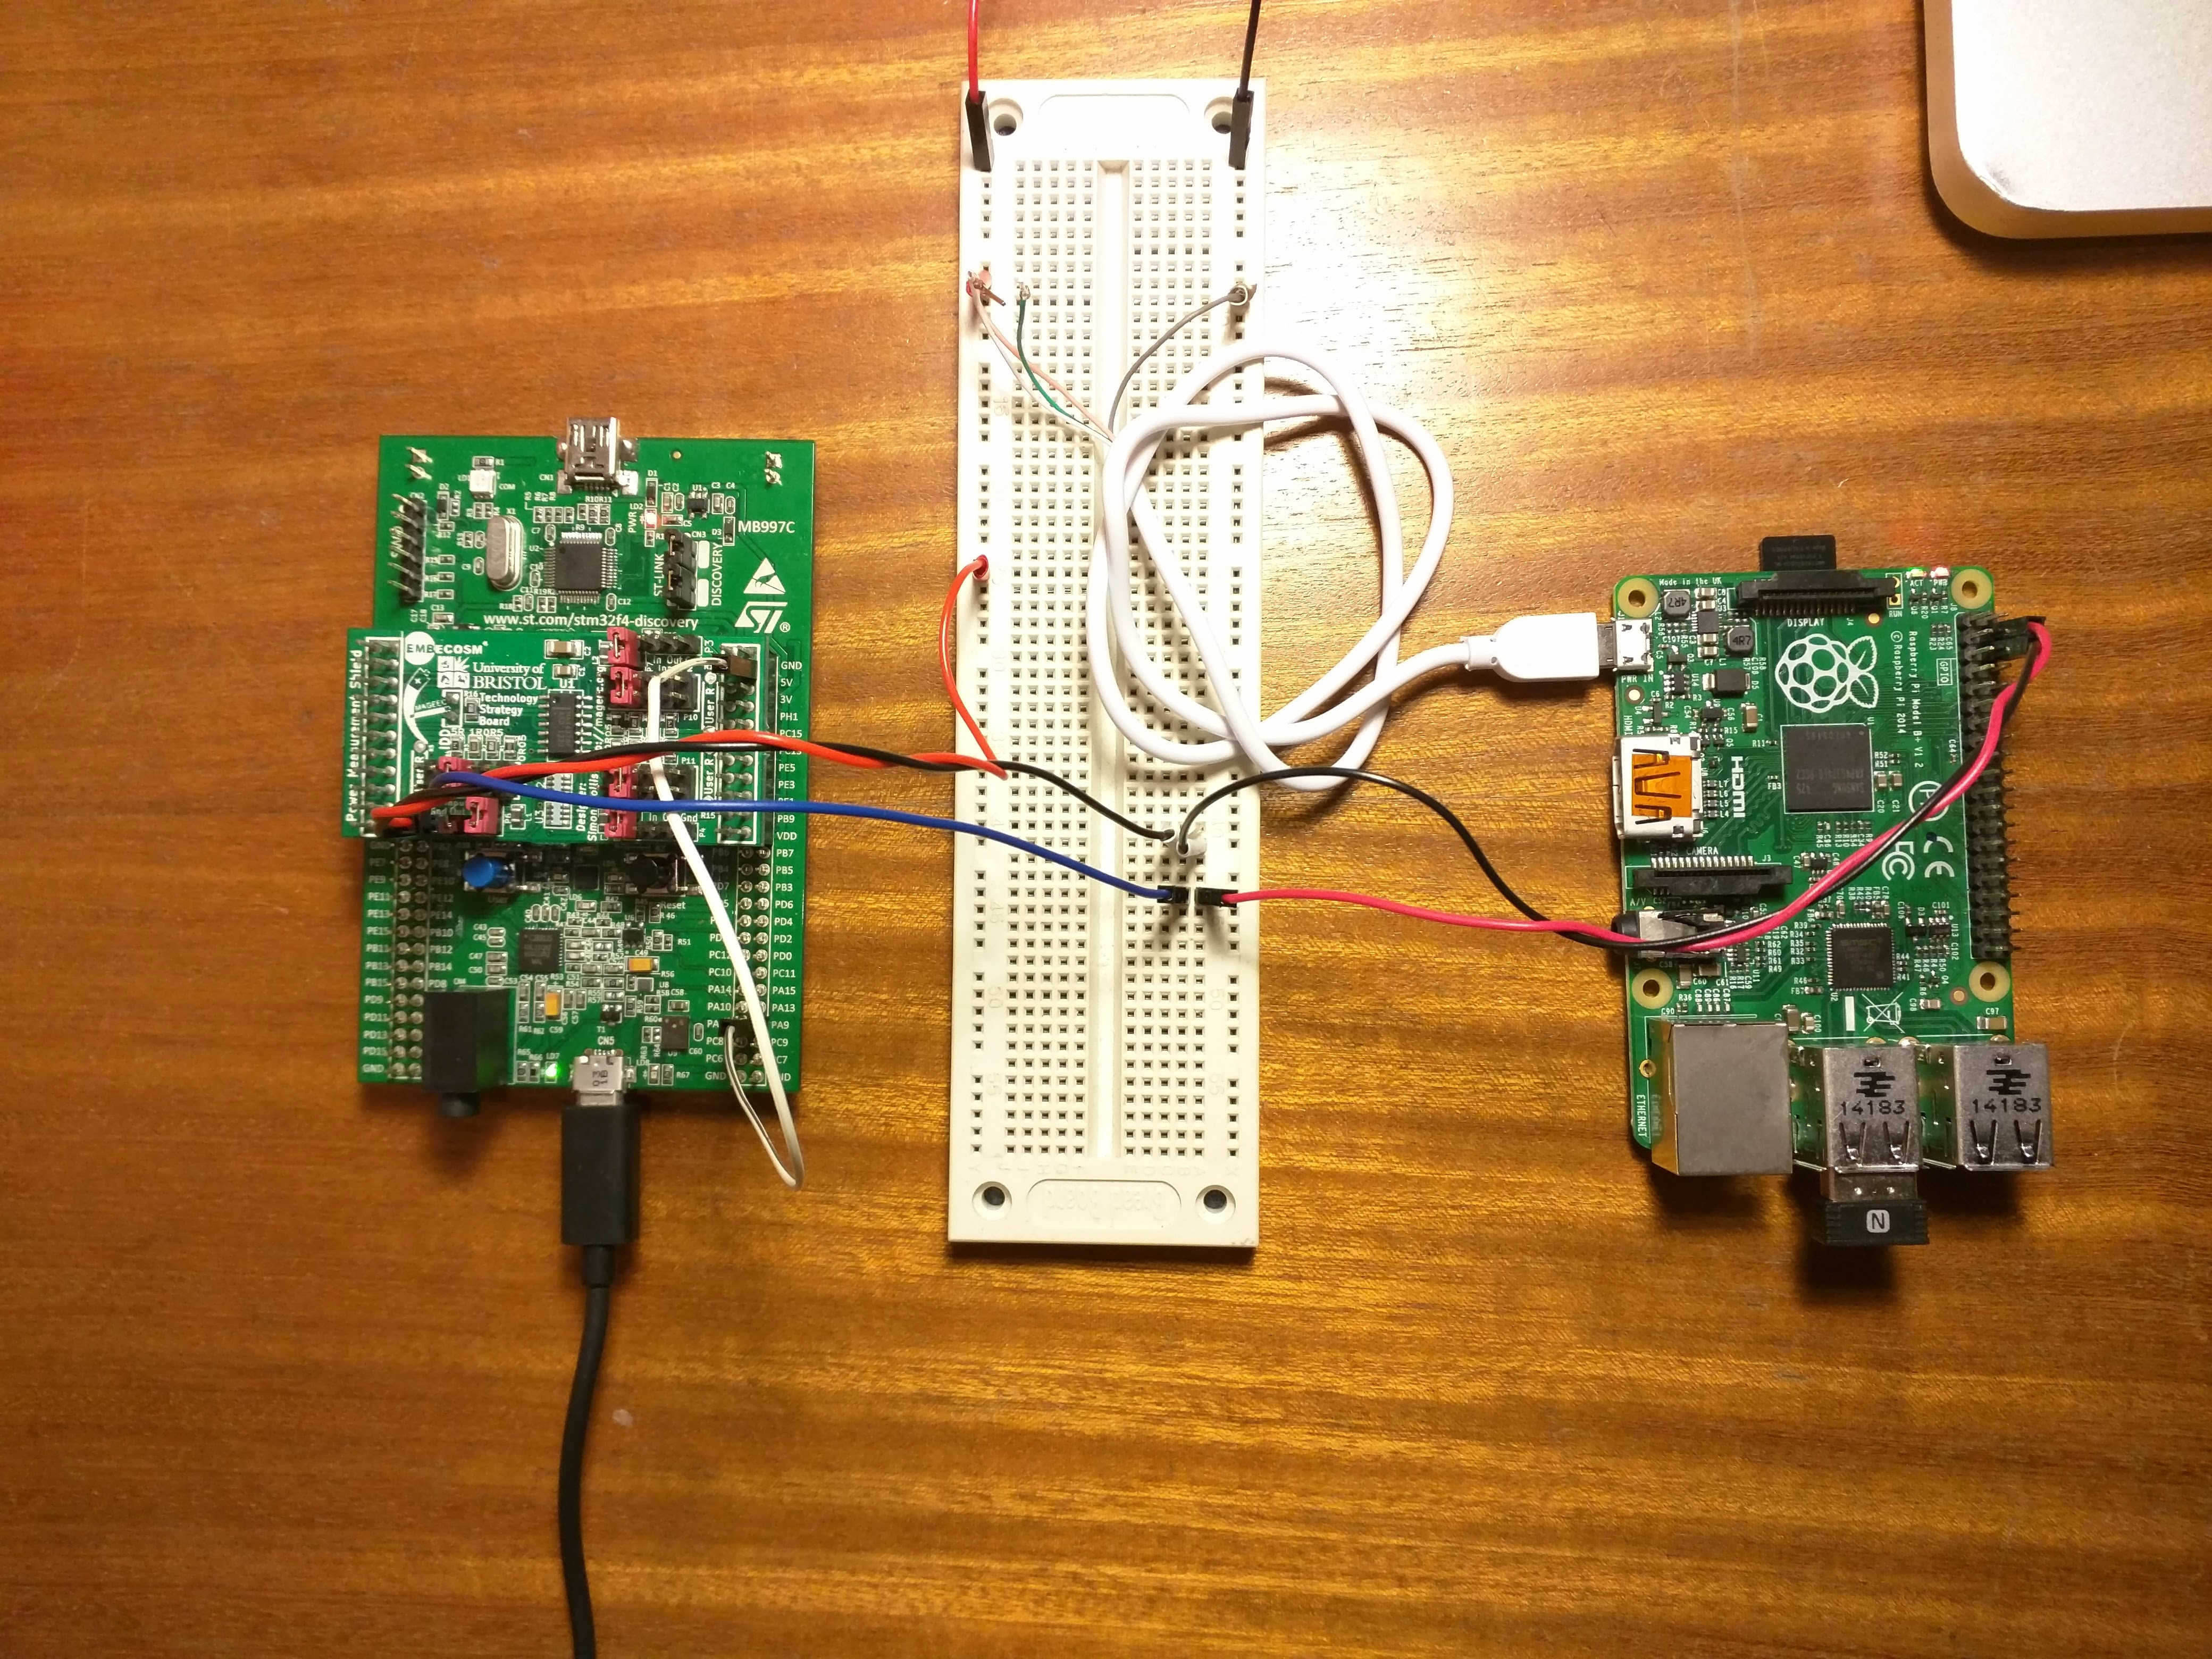
\includegraphics[width=0.6\textwidth]{figures/init_setup}
\end{figure}
\begin{figure}[!ht]
  \caption{The set-up for the whole tower with three nodes connected to the Bristol board.}
  \centering
    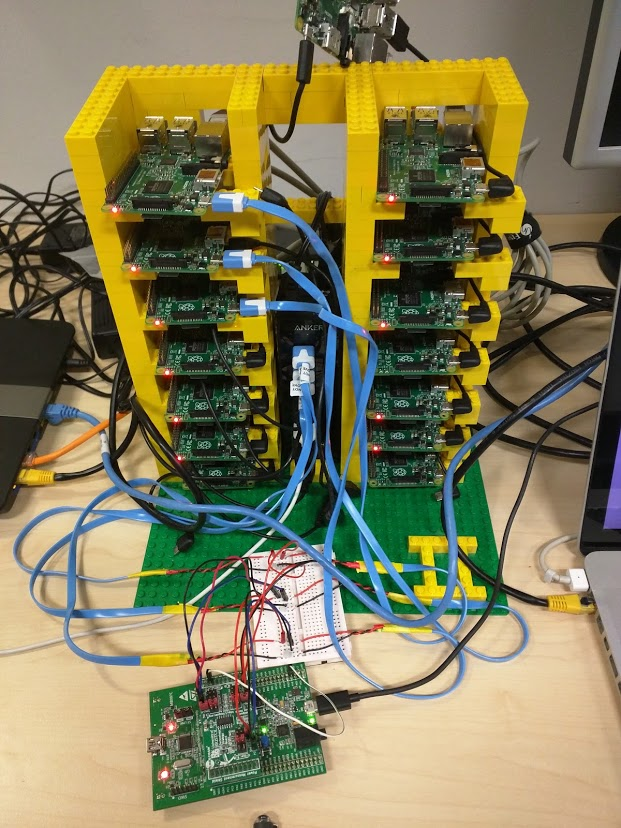
\includegraphics[width=0.6\textwidth]{figures/tower_setup}
\end{figure}
\section{API Server}
\begin{enumerate}
	\item Choice of OS for the Pi
	\item Python chosen as it is most frequently used on the Pi and therefore there is a lot of support and documentation for it.
	\item Flask (and Flask restless) chosen for API. Other options available (Django, Tastypy and Sadman) but Flask is simple and popular and therefore seemed like the right choice.
	\item Chose to use SQLite dabase with Flask SQLalchemy to make database access easier.
\end{enumerate}
\section{Web Client}
\begin{enumerate}
	\item Single Page Application design (rendering and logic done in client which takes processing off server; more responsive websites)
	\item There is a number of frameworks available (Ember.js, ExtJS, React, Knockout) but Angular has a large community and it supports bidirectional data binding, which some of the other frameworks lack
	\item Many front-end frameworks have been adapted to Angular but if they have not it is possible to do it by hand.
\end{enumerate}
\begin{figure}[!ht]
  \caption{TO BE CHANGED! Should make this UML? AngularJS modules and their relationships.}
  \centering
    \includegraphics[width=0.6\textwidth]{figures/client}
\end{figure}
\begin{figure}[!ht]
  \caption{Dashboard wire frame for the web client}
  \centering
    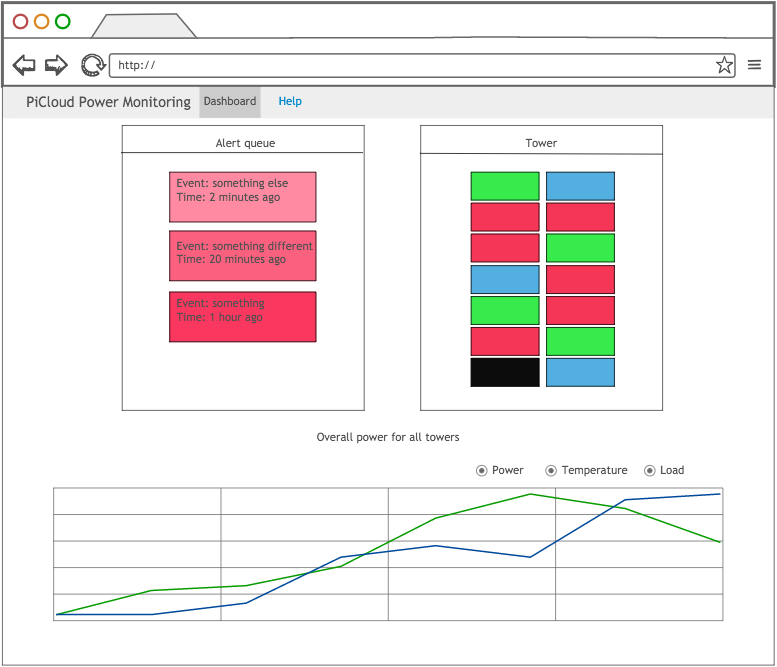
\includegraphics[width=0.8\textwidth]{figures/v2_dashboard}
\end{figure}

%==============================================================================
\chapter{Implementation}
\label{chap_implementation}
\section{Logger Node}
\begin{enumerate}
	\item Logging python (based on MAGEEC pyenergy library)
	\item Database and API
	\item Web client
	\item Salt managing scripts
\end{enumerate}
\section{Minion Nodes}
\begin{enumerate}
	\item Reporting python
\end{enumerate}

%==============================================================================
\chapter{Evaluation}
\section{Testing}
\begin{enumerate}
	\item Python tests for scripts
	\item JavaScript tests(?)
\end{enumerate}
\section{Acceptance Testing}
\begin{enumerate}
	\item Overview of testing scenario
	\item Feedback from testers
	\item Changes in system based on feedback
\end{enumerate}

%==============================================================================
\chapter{Conclusion}
\section{Summary}
\begin{enumerate}
	\item What has been implemented
	\item What the system can do
	\item Comment on usability
\end{enumerate}
\section{Future Work}
\begin{enumerate}
	\item What other features are the next logical step
	\item How do those features fit within the technology stack
\end{enumerate}


%%%%%%%%%%%%%%%%
%              %
%  APPENDICES  %
%              %
%%%%%%%%%%%%%%%%
\begin{appendices}
\chapter{User Stories}
\label{app_user_stories}
\noindent
As an admin \\
I want to see real-time data for the power consumption of the whole tower\\
So that I can identify the total power consumption\\\\
\noindent
As an admin\\
I want to see real-time data for the power consumption for selected nodes (as many as possible)\\
So that I can determine what the power consumption is in various states (idle etc.)\\\\
\noindent
As an admin\\
I want to see real-time CPU temperatures in my cluster in a graph\\
So that I know how they compare with power consumption (on the same graph)\\\\
\noindent
As an admin \\
I want to see real-time CPU loads in my cluster in a graph\\
So that I know how they compare with power consumption (on the same graph)\\\\
\noindent
As an admin\\
I want to be able to change the power, temperature and load sampling frequency\\
So that I can instantaneously have an overview of the data as well as a closer look whenever I want to\\\\
\noindent
As an admin\\
I want to see a real-time diagram representation of the cluster (power, temp, load) with color coding indicating faults or extreme conditions (such as high temperature)\\
So that I have a good overview and can identify which nodes exhibit abnormal behaviour\\\\
\noindent
As an admin\\
I want to see an alert queue that is separate from any other diagram and displays an alert when I need to take action (maybe email alert as well)\\
So that I have a clear indication when I need to respond quickly\\\\
\noindent
As an admin\\
I want to be able to turn off or reboot nodes from the GUI\\
So that I have an easy way of dealing with non-responsive nodes\\\\
\noindent
As an admin
I want to be able to see pods running on each node in real time\\
So I have a better understanding for the level of the node's power consumption\\\\
\noindent
As an admin\\
I want to be able to access log files for power usage (csv)\\
So that I can safely store data and analyse it later\\\\
\noindent
As an admin\\
I want to be able to access the GUI from any browser\\
So that I can view the cluster state from any machine\\\\
\noindent
As an admin \\
I want to be able to see the status of the power measurement board\\
So that I know whether it is providing measurements for the API\\\\
\noindent
As an admin\\
I want to receive data (power, temperature and load) instantaneously\\
So that the graphs update smoothly\\\\

\end{appendices}
%%%%%%%%%%%%%%%%%%%%
%   BIBLIOGRAPHY   %
%%%%%%%%%%%%%%%%%%%%

\bibliographystyle{plain}
\bibliography{bib}

\end{document}
